\section{建立测评指标体系}
    \subsection{确定测评指标}
        \subsubsection{确定测评指标的原则与方法}
            影响读者满意度的因素很多,要根据图书馆工作开展的情况来确定测评指标。指标的列举要尽可能的完整,并且这些指标必须要能够控制和测量,便于进行统计、计算和分析。设计指标时要尽量避免指标间的交叉。如果有交叉,则在问卷的设计上要避免设置相同和很相关的问题。

            指标体系通常是一个多指标、层次化的结构,能够由表及里、深入清晰的表述读者满意度测评指标体系的内涵。每一层次的测评指标都是由上一层测评指标展开的,而上一层次的测评指标体系则是通过下一层的测评指标的测评结果反映出来的 \upcite{彭冬莲2005读者满意度测评方法研究}。
        \subsubsection{确定测评指标}
            影响电子资源建设读者满意度的因素有很多,但是在实际操作中不可能在一次测评中对每一个影响因素都进行测评。因此在本次的课题研究中,根据学院图书馆的实际情况,只对影响电子资源建设读者满意度最主要的因素进行研究和测评 \upcite{彭冬莲2005读者满意度测评方法研究}。

            \begin{table}[h]
                \caption{图书馆各类资源使用率}
                \begin{tabular}{|c|c|c|c|c|c|c|c|}
                    \hline 
                    资源类型 & 纸本图书 & 纸本期刊 & 电子图书 & 电子期刊 & 学位论文数据库 & 专题数据库 & 其他 \\
                    \hline
                    使用率 & 64.0\% & 39.2\% & 35.2\% & 36.8\% & 29.6\% & 15.2\% & 0.04\% \\
                    \hline
                \end{tabular}
            \end{table}

            这里需要一些内容。
            
            \begin{figure}[h]
                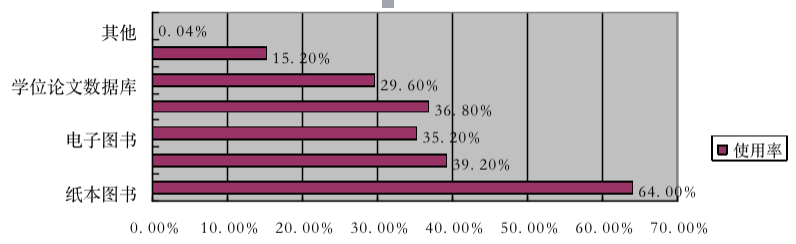
\includegraphics{pic1.png}
                \caption{图书馆各类资源使用率}
            \end{figure}